%%%%%%%%%%%%%%%%%%%%%%%%%%%%%%%%%%%%%%%%%%%%%%%%%%%%%%%%%%%%%%%%%%%%%%%%%%%%%%%%%%%%%
%                        Author: Harshit Prashant Dhanwalkar                        %
%%%%%%%%%%%%%%%%%%%%%%%%%%%%%%%%%%%%%%%%%%%%%%%%%%%%%%%%%%%%%%%%%%%%%%%%%%%%%%%%%%%%%

%-------------------------------------------------------------------------------------
%                    PACKAGES AND OTHER DOCUMENT CONFIGURATIONS                      %
%-------------------------------------------------------------------------------------

\documentclass[fleqn,10pt]{SelfArx} % Document font size and equations flushed left
\usepackage[english]{babel} 
\usepackage{enumitem}

\usepackage{tikz}
\usetikzlibrary{trees, positioning}
\usetikzlibrary{shapes, shadings}
\usepackage{tikz-3dplot}
\usetikzlibrary{3d,shapes.geometric,shadows.blur}
\tikzstyle{vertex}=[draw,fill=black!15,circle,minimum size=20pt,inner sep=0pt]
\tikzstyle{selected edge} = [draw,line width=5pt,-,red!50]

\usepackage{amsmath}
\usepackage{array} % for tables

\usepackage{pgfplots}
\pgfplotsset{compat=1.18}
\tdplotsetmaincoords{60}{115}
\pgfplotsset{compat=newest}

\usepackage{subfig}
%-------------------------------------------------------------------------------------
%                                       COLUMNS                                      %
%-------------------------------------------------------------------------------------
\setlength{\columnsep}{0.55cm} % Distance between the two columns of text
\setlength{\fboxrule}{0.75pt} % Width of the border around the abstract

%-------------------------------------------------------------------------------------
%                                        COLORS                                      %
%-------------------------------------------------------------------------------------
\definecolor{color1}{RGB}{0,0,90} % Color of the article title and sections
\definecolor{color2}{RGB}{0,20,20} % Color of the boxes behind the abstract and headings

%-------------------------------------------------------------------------------------
%                                       EQUATIONS                                    %
%-------------------------------------------------------------------------------------
\usepackage{cancel} % for crossing the word showing it is cancelled or is zero

%-------------------------------------------------------------------------------------
%                                     EQUATIONLINKS                                  %
%-------------------------------------------------------------------------------------
\newcommand{\myeqref}[1]{\textcolor{blue}{\textup{(\getrefnumber{#1})}}}

%-------------------------------------------------------------------------------------
%                                       HYPERLINKS                                   %
%-------------------------------------------------------------------------------------
\usepackage{xcolor}
\usepackage{hyperref}
\usepackage{footnote}

%\newcommand{\myhref}[2]{\href{#1}{\textcolor{blue}{#2}}}
\newcommand{\myhref}[2]{%
  \href{#1}{\textcolor{blue}{#2}}%
  \footnote{\url{#1}}%
}

\usepackage{cleveref}
% Customize cleveref to use "Eq." for equations
\crefname{equation}{Eq.}{Eq.}
\Crefname{equation}{Eq.}{Eq.}

\hypersetup{
	hidelinks,
	colorlinks,
	breaklinks=true,
	urlcolor=color2,
	citecolor=color1,
	linkcolor=color1,
	bookmarksopen=false,
	pdftitle={Title},
	pdfauthor={Author},
}

% ------------------------------------------------------------------------------------
%                                       CUSTOM  SYMBOLS                              %
%-------------------------------------------------------------------------------------
\newcommand{\zbar}{\raisebox{0.2ex}{--}\kern-0.6em Z}

%-------------------------------------------------------------------------------------
%                                       ARTICLE INFORMATION                          %
%-------------------------------------------------------------------------------------
\JournalInfo{Dual Degree Engineering Physics, 8$^{th}$ Semester, 2024} % Journal information
\Archive{Mtech, Earth System Sciences (ESS), 1$^{st}$ year} % Additional notes (e.g. copyright, DOI, review/research article)

\PaperTitle{Lecture Notes on Boundary Layer Meteorology} % Article title

\Authors{Harshit Prashant Dhanwalkar (SC21B164)\textsuperscript{1}*} % Authors
\affiliation{\textsuperscript{1}\textit{MTech, Earth System Sciences (ESS), 1$^{st}$ year, Department of Physics, Indian Institute Of Spacescience and Technology (IIST)}} % Author affiliation
\affiliation{*\textbf{email}: harshitpd1729@gamil.com} % Corresponding author

\Keywords{} % Keywords - if you don't want any simply remove all the text between the curly brackets
\newcommand{\keywordname}{Keywords} % Defines the keywords heading name

%-------------------------------------------------------------------------------------
%                                           ABSTRACT                                 %
%-------------------------------------------------------------------------------------
\Abstract{Notes of Lectures and addional information from books.}

%-------------------------------------------------------------------------------------
%                                            DOCUMENT                                %
%-------------------------------------------------------------------------------------
\begin{document}
\maketitle % Output the title and abstract box
\clearpage
\tableofcontents % Output the contents section
\clearpage
\thispagestyle{empty} % Removes page numbering from the first page
\clearpage

%-------------------------------------------------------------------------------------
%                                       DOCUMENT CONTENTS                           %
%-------------------------------------------------------------------------------------
%\addcontentsline{toc}{section}{Introduction} % Adds this section to the table of contents
%-------------------------------------------------------------------------------------
\section{Lecture 1 09/01/2025}
\subsection{Introduction to Boundary Layer}
The Boundary Layer can be defined as part of  the troposphere that is directly influenced by the presence of the Earth's surface and responds to surface forcings with a time scale of about an hour or less.

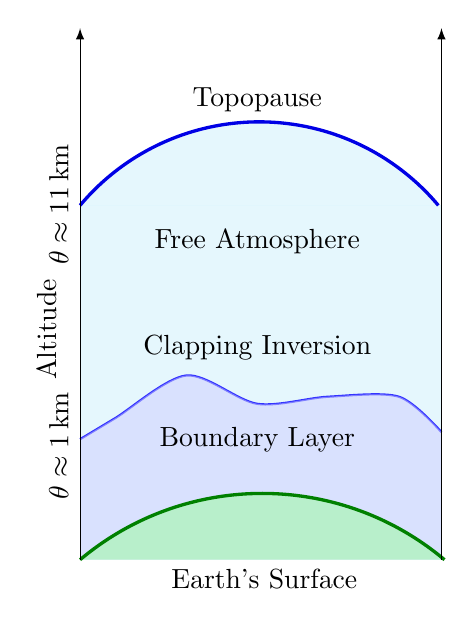
\begin{tikzpicture}[scale=0.9]
	%Free Atmosphere curve
	\fill[cyan!20, opacity=0.5] (-0.5,0) rectangle (4.6,5);
	\fill[cyan!20, opacity=0.5]
	(-0.5,5) arc[start angle=140, end angle=40, radius=3.3cm] -- (4.6,5) -- cycle;
	\draw[very thick, blue!90!black]
	(-0.5,5) arc[start angle=140, end angle=40, radius=3.3cm];
	\node[anchor=north] at (2,4.8) {Free Atmosphere};
	%Topopause curve
	\node[anchor=north] at (2,6.8) {Topopause};
	%Clapping Inversion curve
	\draw[thick,blue!80] plot [smooth] coordinates {(-0.5, 1.7) (0,2) (1,2.6) (2,2.2) (3,2.3) (4,2.3) (4.6,1.8)};
	\fill[blue!20,opacity=0.5] (-0.5,0) -- plot [smooth] coordinates {(-0.5, 1.7) (0,2) (1,2.6) (2,2.2) (3,2.3) (4,2.3) (4.6,1.8)}  -- (4.6,0) -- cycle;
	\node[anchor=north] at (2,3.3) {Clapping Inversion};
	% Boundary layer curve
	\node[anchor=north] at (2,2) {Boundary Layer};
	% Earth's surface
	\fill[green!40,opacity=0.5]
	(2.5-3,0) arc[start angle=130, end angle=50, radius=4cm] -- (2.5,0) -- cycle;
	\draw[very thick, green!50!black, shift={(2.5,0)}]
	(-3,0) arc[start angle=130, end angle=50, radius=4cm];
	\node[below] at (2.1,0) {Earth's Surface};
	% Axis label
	\draw[-latex] (-0.5,0) -- (-0.5,7.5);
	\node[above, rotate=90] at (-0.7,3.25) {Altitude};
	\draw[-latex] (4.6,0) -- (4.6,7.5);
	% Labels
	\node[anchor=east, rotate=90] at (-0.8,6) {\(\theta \approx 11 \, \mathrm{km}\)};
	\node[anchor=east, rotate=90] at (-0.8,2.5) {\(\theta \approx 1 \, \mathrm{km}\)};
\end{tikzpicture}

\subsection{Boundary layer forcing mecchanism}
What physical process modify boundary layer air parcel?
\begin{enumerate}[noitemsep]
	\item Heat transfer to.from the ground.
	\item Frictional drag.
	\item Evaporation/transpiration.
	\item Terrain-induced flow modification.
	\item Pollution emission.
\end{enumerate}

\subsection{Types of air flow or wind}
Air flow or wind can be decomposed into following 3 types:
\begin{enumerate}[noitemsep]
	\item \textbf{Mean Wind} $(\bar{u}, \bar{v}, \bar{w})$: Represents the average wind components in the horizontal ($\bar{u}, \bar{v}$) and vertical ($\bar{w}$) directions. It is important for the horizontal transport of quantities such as moisture, heat, momentum, and pollutants, a process known as advection.
	\item \textbf{Waves}: Atmospheric waves, such as gravity waves, occur mostly at night in the nocturnal boundary layer (NBL). They can influence the structure of the boundary layer and the transport of energy.
	\item \textbf{Turbulence}: The vertical transport of moisture, heat, momentum, and pollutants is primarily dominated by turbulence, which is characterized by chaotic and irregular motion.
\end{enumerate}

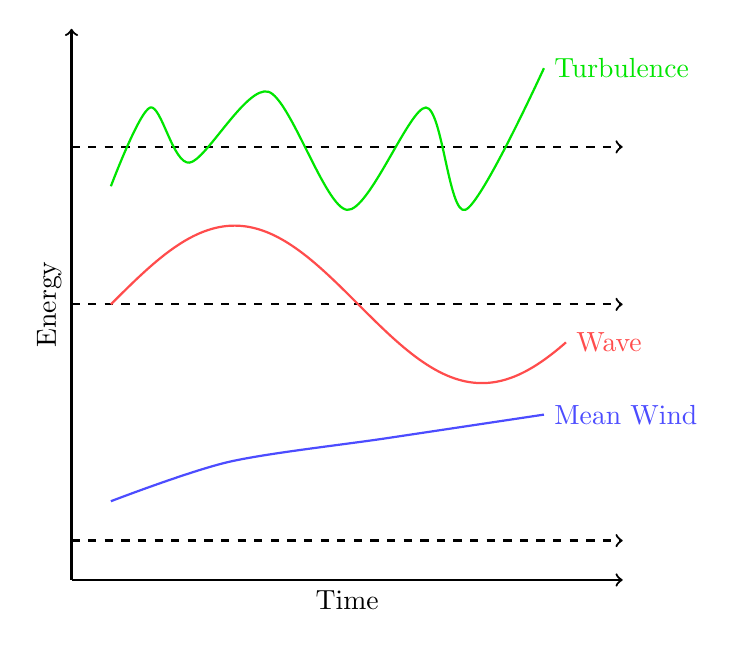
\begin{tikzpicture}[smooth, thick]
	% Axes
	\draw[dashed,->] (0,0.5) -- (7,0.5);
	\draw[dashed,->] (0,3.5) -- (7,3.5);
	\draw[dashed,->] (0,5.5) -- (7,5.5);
	\draw[->] (0,0) -- (7,0);
	\node[below] at (3.5,0) {Time};
	\draw[->] (0,0) -- (0,7);
	\node[above, rotate=90] at (0,3.5) {Energy};
	% Mean Wind (Offset by +2 for vertical distance)
	\draw[blue!70] plot coordinates {(0.5,1) (2,1.5) (4,1.8) (6,2.1)}
	node[anchor=west] {Mean Wind};
	% Wave (Sine curve, offset by +4)
	\draw[red!70] plot[domain=0.5:6.28,samples=100]
	({\x},{3.5 + sin((\x - 0.5) r)})
	node[anchor=west] {Wave};
	% Turbulence (Offset by +6)
	\draw[green!90!black] plot coordinates {(0.5,5) (1,6) (1.5,5.3) (2.5,6.2) (3.5,4.7) (4.5,6) (5,4.7) (6,6.5)}
	node[anchor=west] {Turbulence};
\end{tikzpicture}

\subsection{Eddies}
Eddies are formed due to the interaction of currents with obstacles like coastlines, underwater topography, or other currents, as well as from the instability of larger current systems.
Eddies exhibit a rotational flow pattern, either clockwise or counterclockwise.
Eddies can vary from size 100 to 3000 metres and also can exists as small as few millimetres.
Small eddies might last for seconds to minutes, while larger oceanic eddies can persist for weeks, months, or even years.

\subsection{Turbulence Generation Mechanisms}
\begin{itemize} [noitemsep]
	\item \textbf{Solar Heating}: Solar heating generates thermals, which are essentially larger eddies that drive turbulence in the atmospheric boundary layer.
	\item \textbf{Wind Shear}: Variations in wind speed or direction with height create wind shear, which is a significant source of turbulence.
	\item \textbf{Obstacle-Induced Flow}: Deflected flow around obstacles such as trees, buildings, or other structures generates turbulent eddies downstream of these obstacles, creating turbulent wakes.
\end{itemize}

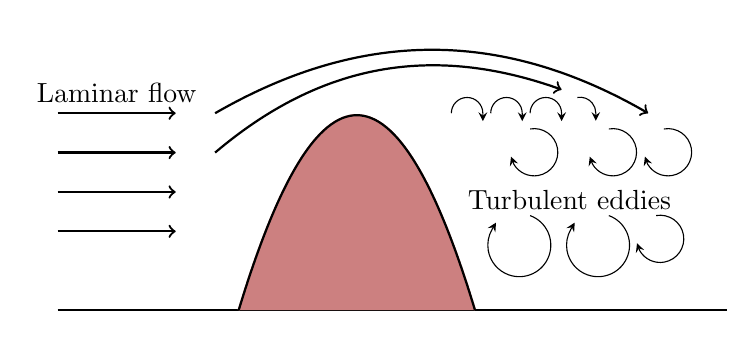
\begin{tikzpicture}
	% Ground
	\draw[thick] (-1,0) -- (7.5,0);
	% Obstacle
	\filldraw[thick, red!60!black!50] (1.3,0) .. controls (2.3,3.3) and (3.3,3.3) .. (4.3,0);
	\draw[thick]  (1.3,0) .. controls (2.3,3.3) and (3.3,3.3) .. (4.3,0);
	% Laminar flow arrows
	\draw[->,thick] (-1,2.5) -- (0.5,2.5) node[midway,above] {Laminar flow};
	\draw[->,thick] (-1,2) -- (0.5,2);
	\draw[->,thick] (-1,1.5) -- (0.5,1.5);
	\draw[->,thick] (-1,1) -- (0.5,1);
	% b/w laminar and eddies
	\draw[->,thick] (1,2) to[bend left] (5.4,2.8);
	\draw[->,thick] (1,2.5) to[bend left] (6.5,2.5);
	% Turbulent eddies
	\foreach \x in {4, 4.5, 5}
	\draw [>=stealth,->] (\x,2.5) arc (180:0:.2cm) -- +(270:0.1cm);
	\draw [>=stealth,->] (5.6,2.7) arc (100:0:.2cm) -- +(270:0.1cm);
	\foreach \x in {5, 6, 6.7}
	\draw [>=stealth,->] (\x,2.3) arc (100:-150:.3cm) -- +(110:0.1cm);
	\draw [>=stealth,->] (6.6,1.2) arc (100:-150:.3cm) -- +(110:0.1cm);
	\foreach \x in {5,6}
	\draw [>=stealth,->] (\x,1.2) arc (70:-210:.4cm) -- +(60:0.1cm);
	\node at (5.5,1.4) {Turbulent eddies};
\end{tikzpicture}

Large eddies will break into smaller eddies after which small eddies dissipates from K.E. to thermal energy.

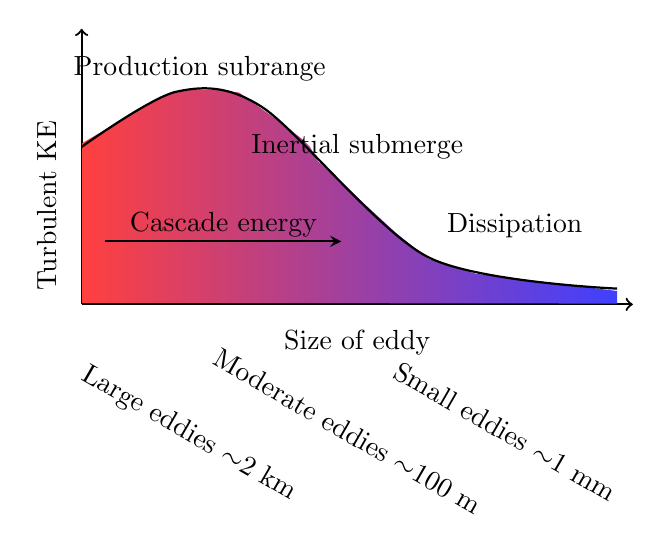
\begin{tikzpicture}
	% Axes
	\draw[thick,->] (0,0) -- (7,0);
	\node[below] at (3.5,-0.2) {Size of eddy};
	\draw[thick,->] (0,0) -- (0,3.5);
	\node[above, rotate=90] at (-0.2,1.25) {Turbulent KE};
	% Curve
	%\filldraw[blue!50, thick, smooth](0.03,0.04) -- plot coordinates {(0.03,2) (1.2,2.7) (2.3,2.5) (4.4,0.6) (6.8,0.2)} -- (6.8,0.04) -- cycle;
	\shade[left color=red!75, right color=blue!75] (0.01,0.02) -- plot coordinates {(0.01,2.05) (1,2.625) (1.25, 2.71) (1.5,2.73) (1.75,2.72) (2,2.69) (2.5,2.33) (2.8,2.1) (2.9,2) (3,1.82) (4,0.9) (4.4,0.58) (5,0.39) (6.8,0.17)} -- (6.8,0.01) -- cycle;
	\draw[thick,smooth] plot coordinates {(0,2) (1.2,2.7) (2.3,2.5) (4.4,0.6) (6.8,0.2)};
	% Labels
	\node at (1.5,3) {Production subrange};
	\node at (3.5,2) {Inertial submerge};
	\node at (5.5,1) {Dissipation};
	\draw[thick, -stealth] (0.3,0.8) -- (3.3,0.8);
	\node[below] at (1.8,1.3) {Cascade energy};
	% Size labels
	\node[below, rotate=-30] at (1.5,-1.4) {Large eddies $\sim$2 km};
	\node[below, rotate=-30] at (3.5,-1.4) {Moderate eddies $\sim$100 m};
	\node[below, rotate=-30] at (5.5,-1.4) {Small eddies $\sim$1 mm};
\end{tikzpicture}

\clearpage

\section{Leture 2 15/01/2025}
\subsection{Taylor's Hypothesis}
\begin{itemize}[noitemsep]
	\item When studying atmospheric boundary layer (ABL), It is not easy to create a snapshot of turbulance in the Atmosphere.
	\item Hence it is easier and cheaper to make measurements of point in the atmoshpere for a longer time, then an instantaneous snapshot.
	\item So we just consider the atmoshpere is frozen.
	\item \textbf{\textit{Taylor suggested that turbulence can be considered frozen as it advects past sensor.}}
\end{itemize}

\begin{figure}[h!]
	\centering
	\resizebox{0.5\textwidth}{!}{
		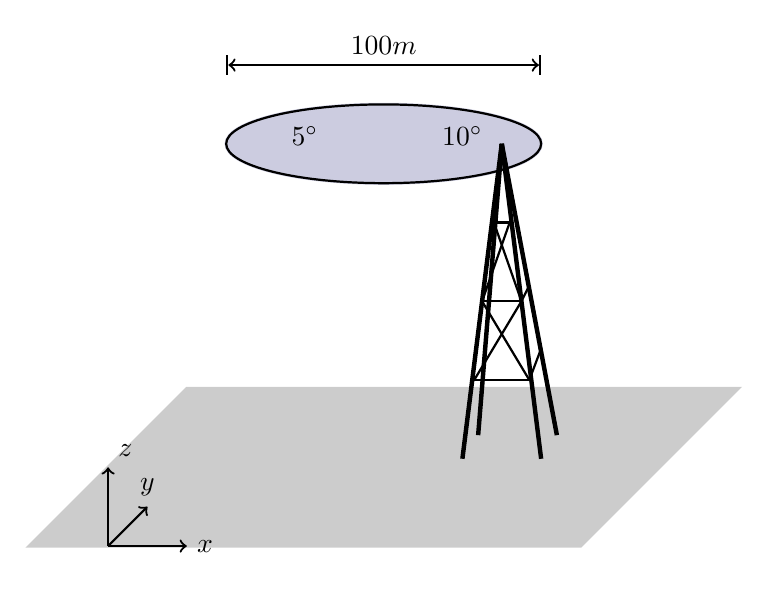
\begin{tikzpicture}
			% ground
			\begin{scope}[yshift=-60,yslant=0,xslant=1]
				\filldraw[black!20,very thick] (-7,1) rectangle (0,3);
				\draw[->, thick] (-6, 1) -- (-5, 1) node[right] {\( x \)};
				\draw[->, thick] (-6, 1) -- (-6, 1.5) node[above] {\( y \)};
				\draw[->, thick] (-6, 1) -- (-7, 2) node[above right] {\( z \)};
			\end{scope}
			% eddy
			\filldraw[black!60!blue!20, very thick] (-1.5, 4) ellipse [x radius=2, y radius=0.5];
			\draw[thick] (-1.5, 4) ellipse [x radius=2, y radius=0.5];
			\node at (-2.5,4.1) {$5^\circ$};
			\node at (-0.5,4.1) {$10^\circ$};
			\draw[|<->|, thick] (-3.5, 5) -- (0.5, 5) node[midway, above] {$100m$};
			% Slant lines
			\draw[ultra thick] (-0.5, 0) -- (0, 4);
			\draw[ultra thick] (-0.3, 0.3) -- (0, 4);
			\draw[ultra thick] (0.5, 0) -- (0, 4);
			\draw[ultra thick] (0.7, 0.3) -- (0, 4);
			% Horizontal lines
			\draw[thick] (-0.35, 1) -- (0.35, 1);
			\draw[thick] (-0.25, 2) -- (0.25, 2);
			\draw[thick] (-0.10, 3) -- (0.10, 3);
			\draw[thick] (0.35, 1) -- (0.5, 1.4);
			\draw[thick] (0.25, 2) -- (0.35, 2.2);
			% Crosses at intersections
			\draw[thick] (-0.35, 1) -- (0.25, 2);
			\draw[thick] (-0.25, 2) -- (0.35, 1);
			\draw[thick] (-0.10, 3) -- (0.25, 2);
			\draw[thick] (-0.25, 2) -- (0.10, 3);
		\end{tikzpicture}
	}
\end{figure}

\begin{figure}[h!]
	\centering
	\resizebox{0.5\textwidth}{!}{
		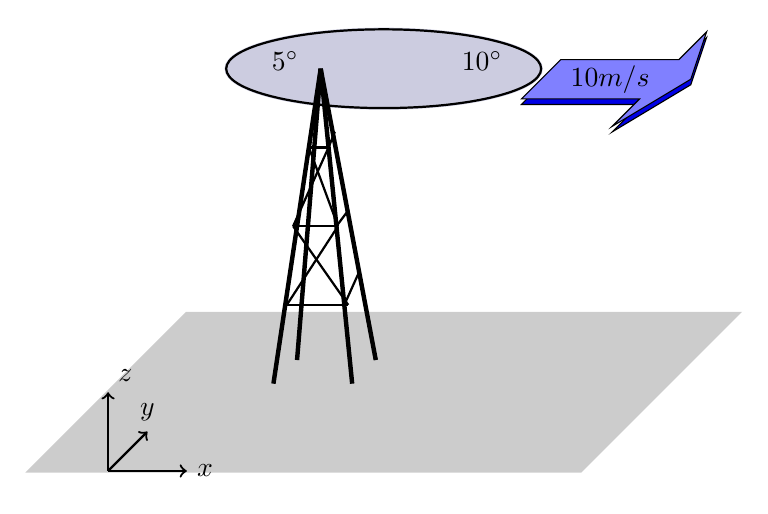
\begin{tikzpicture}
			% ground
			\begin{scope}[yshift=-60,yslant=0,xslant=1]
				\filldraw[black!20,very thick] (-5,1) rectangle (2,3);
				\draw[->, thick] (-4, 1) -- (-3, 1) node[right] {\( x \)};
				\draw[->, thick] (-4, 1) -- (-4, 1.5) node[above] {\( y \)};
				\draw[->, thick] (-4, 1) -- (-5, 2) node[above right] {\( z \)};
			\end{scope}
			\begin{scope}[yshift=108,yslant=0,xslant=1]
				\draw[fill=blue!90!black] (2.5,0.25) --  (4,0.25) coordinate (f1)
				-- (4,0.6) coordinate (f2) -- (4.4,0) coordinate (f3)
				-- (4,-0.6) coordinate (f4) -- (4,-0.25) coordinate (f5)
				-- (2.5,-0.25) coordinate (f6) -- cycle;
			\end{scope}
			\begin{scope}[yshift=110,yslant=0,xslant=1]
				\draw[fill=blue!50] (2.5,0.25) --  (4,0.25) coordinate (f1)
				-- (4,0.6) coordinate (f2) -- (4.4,0) coordinate (f3)
				-- (4,-0.6) coordinate (f4) -- (4,-0.25) coordinate (f5)
				-- (2.5,-0.25) coordinate (f6) -- cycle;
				\path (2, 0) -- (4, 0) node[pos=1, font=\sffamily, anchor=east]{$10m/s$};
			\end{scope}
			% eddy
			\filldraw[black!60!blue!20, very thick] (0.5, 4) ellipse [x radius=2, y radius=0.5];
			\draw[thick] (0.5, 4) ellipse [x radius=2, y radius=0.5];
			\node at (-0.75,4.1) {$5^\circ$};
			\node at (1.75,4.1) {$10^\circ$};
			% Slant lines
			\draw[ultra thick] (-0.9, 0) -- (-0.3, 4);
			\draw[ultra thick] (-0.6, 0.3) -- (-0.3, 4);
			\draw[ultra thick] (0.1, 0) -- (-0.3, 4);
			\draw[ultra thick] (0.4, 0.3) -- (-0.3, 4);
			% Horizontal lines
			\draw[thick] (-0.73, 1) -- (0.05, 1);
			\draw[thick] (-0.65, 2) -- (-0.08, 2);
			\draw[thick] (-0.45, 3) -- (-0.2, 3);
			\draw[thick] (0, 1) -- (0.18, 1.4);
			\draw[thick] (-0.1, 2) -- (0.05, 2.2);
			\draw[thick] (-0.2, 3) -- (-0.12,3.2);
			% Crosses at intersections
			\draw[thick] (-0.73, 1) -- (-0.08, 2);
			\draw[thick] (-0.65, 2) -- (0.05, 1);
			\draw[thick] (-0.65, 2) -- (-0.2, 3);
			\draw[thick] (-0.45, 3) -- (-0.08, 2);
		\end{tikzpicture}
	}
\end{figure}

\begin{align*}
	\frac{\partial T}{\partial x} = 0.05 \text{K/m,} \quad \frac{\partial T}{\partial t} = -0.5 \text{K/s} \\
	\underbrace{\cancel{\frac{D T}{D t}}}_{\substack{\text{Total derivative = 0}                           \\ \text{ (Taylor's hypothesis)}}} =\underbrace{\frac{\partial T}{\partial t}}_{\text{Local derivative}} + \underbrace{u\frac{\partial T}{\partial x}}_{\text{Advective term}}
\end{align*}

\subsection{Virtual Potential Temperature}
Virtual potential temperature:
\begin{equation}
	\theta_v = \theta(1+0.61r)
	\label{eq:virtualpotentialtemp}
\end{equation}
Virtual temperature:
\begin{equation}
	T_v = T(1+0.61r)
	\label{eq:virtualtemp}
\end{equation}

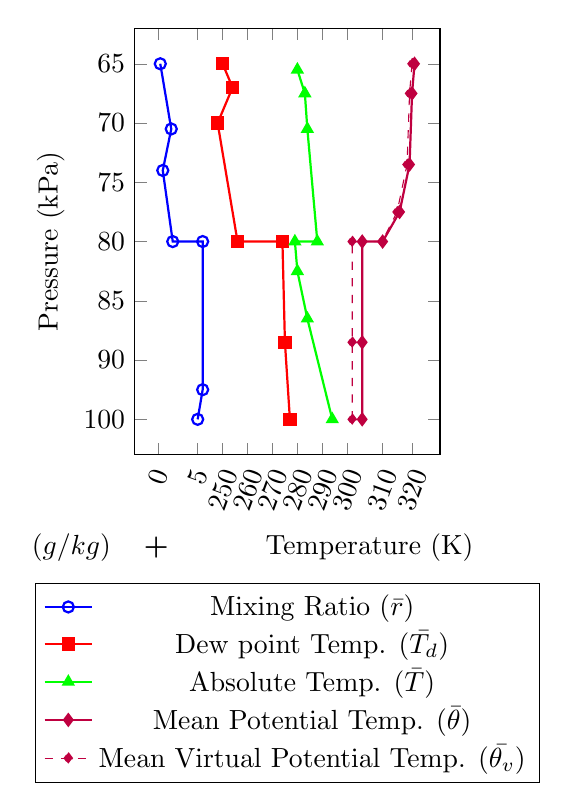
\begin{tikzpicture}
	\begin{axis}[
			%axis lines=middle,
			xlabel={\hspace{-1cm} ($g/kg$) \hspace{0.3cm}$\textbf{+}$ \hspace{1cm} Temperature (K)},
			ylabel={Pressure (kPa)},
			legend style={at={(0.5,-0.3)}, anchor=north},
			width=0.45\textwidth, height=7cm,
			xtick=      {0.2, 1, 1.5, 2,    2.5, 3,   3.5,  4,   4.7,   5.3},
			xticklabels={0,   5, 250, 260,  270, 280, 290,  300, 310, 320},
			ytick=	    {0,   1,  2,  3,  4,  5,  6},
			yticklabels={100, 90, 85, 80, 75, 70, 65},
			xticklabel style={rotate=70},
			% yticklabel style={rotate=0}
		]
		]
		\addplot[mark=o, blue, thick] coordinates {
				(1,0) (1.1,0.5) (1.1,3) (0.5,3) (0.3,4.2) (0.47,4.9) (0.25,6)
			};
		\addlegendentry{Mixing Ratio ($\bar{r}$)}

		\addplot[mark=square*, red, thick] coordinates {
				(2.85,0) (2.75,1.3) (2.7,3)  (1.8,3) (1.4,5) (1.7,5.6) (1.5,6)
			};
		\addlegendentry{Dew point Temp. (${\bar{T_d}}$)}

		\addplot[mark=triangle*, green, thick] coordinates {
				(3.7,0) (3.2,1.7) (3,2.5) (2.95,3) (3.4,3) (3.2,4.9) (3.15,5.5) (3.0,5.9)
			};
		\addlegendentry{Absolute Temp. (${\bar{T}}$)}

		\addplot[mark=diamond*, purple, thick] coordinates {
				(4.3,0) (4.3,1.3) (4.3,3) (4.71,3) (5.05,3.5) (5.25,4.3) (5.3,5.5) (5.35,6)
			};
		\addlegendentry{Mean Potential Temp. (${\bar{\theta}}$)}

		\addplot[mark=diamond*, purple, dashed] coordinates {
				(4.1,0) (4.1,1.3) (4.1,3) (4.7,3) (5,3.5) (5.2,4.3) (5.25,5.5) (5.3,6)
			};
		\addlegendentry{Mean Virtual Potential Temp. (${\bar{\theta_v}}$)}
	\end{axis}
\end{tikzpicture}

\begin{question}{}
	Given 25$^\circ$C termperature, mixing ratio $\bar{r}$ is 20$g/kg$, measured Pressurere at 900$hPa$, find virtual potential temperature.
\end{question}
\begin{answer}{}
	Solution:\begin{align*}
		\theta            & = T \times \Big(\frac{1000}{P}\Big)^{0.286}      \\
		                  & = 298 \times \Big(\frac{1000}{900}\Big)^{0.286}  \\
		                  & = 332.222 K                                      \\
		\theta_v          & = \theta \times \big(1 + 0.61r \big)             \\
		                  & = 332.22 \times \big(1 + 0.61 \times 0.025 \big) \\
		                  & = 336.273 K                                      \\
		\theta_v - \theta & \approx 4.05 K
	\end{align*}
\end{answer}
\end{document}
